\chapter{Desarrollo}\label{chapter:implementation}

El sistema propuesto es una aplicación web, la cual expondrá una API\footnote{Una interfaz de programación de aplicaciones (API por sus siglas en inglés) es una forma en que dos o más programas de computadora se comunican entre sí.} que permitirá manejar el modelo y la sincronización de los datos de interés para el cuidado de las mascotas, haciendo uso del framework\footnote{Un framework es una herramienta que proporciona componentes listos para usar o soluciones personalizables para acelerar el desarrollo de software.} ASP.NET Web API\footnote{Es un framework para crear servicios HTTP a los que se puede acceder desde cualquier cliente, incluidos navegadores y dispositivos móviles.}. El framework .NET permite, de manera simple y elegante, la implementación de aplicaciones web rápidas y confiables. Otra de las características que agregan valor a este framework es que permite desarrollar, compilar y ejecutar aplicaciones en distintas plataformas, facilitando el desarrollo de la aplicación y la configuración del entorno de desarrollo. Se usó la herramienta Entity Framework Core, un ORM que facilita el acceso a datos, en este caso en una base de datos de SQL Server.
\newline

En este capítulo estaremos analizando las características de las herramientas utilizadas en este proyecto, con las que se integra .NET.

\section{El lenguaje C\#:}

\brackcite{albahari2021c}C\# es un lenguaje de programación de propósito, fuertemente tipado y orientado a objetos, diseñado por un equipo dirigido por Anders Hejlsberg. El lenguaje está orientado a la productividad, por lo que busca un balance entre simplicidad, expresividad y rendimiento. Posee Garbage Collection\footnote{Es una forma de gestión automática de la memoria.}, una de las características mas deseadas en el desarrollo de software debido a la complejidad que puede alcanzar manejar los recursos computacionales usados en un proyecto de gran escala. El tipado estático es otra de las características que lo hace un lenguaje seguro. El chequeo de tipos ocurre en tiempo de compilación, reduciendo así los errores de tipado que pueden llegar a ser comunes en otros lenguajes.
\newline

Otro de los motivos de escoger C\# como lenguaje para desarrollar nuestra aplicación es la documentación. Microsoft ha puesto un gran esfuerzo en este aspecto, por lo que tenemos acceso gratuito a documentación escrita por el mismo equipo de desarrollo del lenguaje, así como de la gran comunidad de desarrolladores independientes que le aportan mejorías constantemente. C\# es sin duda alguna una de las opciones más robustas en cuanto a desarrollo de software con fines comerciales.

\section{Objet Relational Mapper(ORM) Entity Framework Core:}

\brackcite{schwdern}En el mundo de la computación actual aún usamos bases de datos relacionales, esto es debido a que su eficacia para representar y gestionar información nos permite modelar elementos de la vida real con relativa facilidad.

En la POO\footnote{Programación Orientada a Objetos: Es un paradigma de programación que se basa en el concepto de crear un modelo del problema de destino en sus programas.} nos apoyamos en los objetos para representar la información. Esta forma de representación es lo suficientemente expresiva para facilitarnos la definición de cualquier entidad real que se encuentre en un problema computacional. El problema en este caso, viene dado por la persistencia, la forma en la que almacenamos objetos limita la eficacia de su gestión.
\newline

Los ORM nacen con el fin de que los programadores puedan beneficiarse a la vez del poder expresivo de la POO y la eficacia del manejo de datos característica de las bases de datos relacionales. Ahora los desarrolladores pueden concentrarse en el desarrollo orientado a objetos sin necesidad de preocuparse de tareas menos interesantes, como consultas básicas de crear, actualizar, eliminar y leer datos de una base de datos relacional. El decremento de errores  introducidos durante el desarrollo de software es considerable cuando se usa un ORM.
\newline

El ORM Entity Framework Core(EF Core) es un framework de acceso a datos, ligero y de código abierto desarrollado sobre (glocary)ADO.NET. Como está escrito en .NET Core es posible ejecutarlo en varios sistemas operativos, incluyendo sistemas operativos móviles como iOS y Android, estos últimos solo soportan acceso a base de datos locales como SQLite\footnote{Es una biblioteca escrita en el lenguaje C que implementa un motor de base de datos SQL pequeño, rápido, autónomo, de alta confiabilidad y con todas gran variedad de funcionalidades.}. \brackcite{ajcvickers2022Nov}La versión gratuita del framework provee soporte para varias bases de datos relacionales como:


\begin{itemize}
	\item SQL Server.
    \item SQLite.
    \item Base de datos en memoria de EF Core.
    \item API de SQL de Azure Cosmos DB.
    \item PostgreSQL.
    \item MariaDB.
    \item MySQL.
    \item Archivos de Microsoft Access.
    
\end{itemize}

Varias de las ventajas que podemos percibir de usar EF Core en el desarrollo de software son:

\begin{itemize}
	\item \textbf{Seguimiento de entidades:} Permite a EF Core saber cuando una entidad ha sido modificada. De esta forma el cambio de estado de un objeto siendo seguido por EF Core es automáticamente agregado al conjunto de operaciones a ejecutar en la base de datos cuando guardamos los cambios hechos.
    \item \textbf{Generación de consultas:} EF Core genera consultas SQL eficientes en la mayoría de los escenarios. En caso de que la consulta generada automáticamente no tenga desempeño esperado, podemos entonces escribir la consulta SQL directamente nosotros para que sea ejecutada en la base de datos.
    \item \textbf{Proyecciones usando Select:} Podemos generar proyecciones para nuestras consultas haciendo uso del método Select de \textbf{LINQ}\footnote{Language Integrated Query es un componente de Microsoft .NET Framework que agrega capacidades de consulta de datos nativos a los lenguajes de .NET.}. Evitando leer campos que pueden ser ignorados en algunos escenarios, reducimos la carga de información leída, mejorando así el rendimiento de nuestras consultas.
    \item \textbf{Ejecución de grupos de consultas:} EF Core agrupa las consultas de actualización, inserción y eliminación en grupos para ser ejecutados en la base de datos. Usando esta estrategia disminuimos la cantidad de conexiones necesarias con la base de datos, aumentando así el rendimiento del software.
    
\end{itemize}

\section{Autorización con Bearer Tokens:}
\brackcite{Jones2012Oct}Los Bearer Tokens nacieron como parte del estándar \textbf{rfc6750}\footnote{Esta especificación describe cómo usar Bearer tokens en consultas HTTP para acceder a recursos protegidos por OAuth 2.0. https://www.rfc-editor.org/rfc/rfc6750}.  En el caso de nuestra aplicación, el cliente principal es una aplicación móvil. Una de las cuestiones importantes en este aspecto es cómo mantener la sesión iniciada por un usuario para que este no deba autenticarse constantemente para acceder a los recursos de la app. Haciendo uso de los Bearer Tokens podemos proporcionar a la app cliente de forma segura a través del protocolo HTTPS un token de vida finita. Este token siendo incluido en el encabezado nos permite comprobar de forma segura que se trata de un cliente autorizado a acceder a un recurso específico. Este tipo de autorización es segura ya que la vida de dicho token es corta y esto disminuye las filtraciones de seguridad.
\begin{figure}[H]
	\centering
	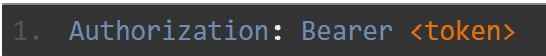
\includegraphics[width = 10cm]{Graphics/bearer_token.jpg}
	\caption{Encabezado de Bearer Toke. }
	\label{fig:bearer_tokne}
\end{figure}

\section{Despliegue:}

\brackcite{carzaniga1998characterization}El despliegue de un sistema es, de manera informal, es el conjunto de procesos a llevar a cabo para poder hace que un software esté disponible para su uso. Aunque esta definición informal define de forma bastante intuitiva el objetivo de despliegue, la estrategia adoptada está vinculada a las especificidades del proyecto que se quiere desplegar. Debido a esto, el desarrollo de una estrategia varía de un sistema a otro.
\newline


\brackcite{pressman2019software}El proceso de despliegue está caracterizado por tres actividades fundamentales: entrega, soporte y retroalimentación. Debido a que en la actualidad los sistemas desarrollados son de carácter incremental y evolutivo, el despliegue ocurre no solo una vez, sino que se lleva a cabo varias veces durante la vida útil del software. Las etapas se pueden caracterizar de la siguiente forma:

\begin{itemize}
	\item \textbf{Entrega:} Cada ciclo de entrega provee al cliente y a los usuarios nuevas características funcionales, incrementando así la operabilidad del software.
    \item \textbf{Soporte:} En los ciclos de soporte se provee documentación y asistencia humana sobre todas las funcionalidades y característica introducidas en todos los ciclos hechos hasta la actualidad.
    \item \textbf{Retroalimentación:} El equipo de desarrollo recibe información y guías para realizar modificaciones de las funcionalidades, características y estrategias a tener en cuenta para la próxima etapa de desarrollo.
    
\end{itemize}

El trabajo requerido para desplegar una aplicación solía ser engorroso y podía requerir gran experticia para lograrlo correctamente. Era un proceso propenso a errores y las actualizaciones eran igual de costosas, lo que hacía más difícil la actualización del sistema y restringía bastante la libertad de los desarrolladores. 
\newline

En la actualidad se ha popularizado el uso de contenedores como substituto de las máquinas virtuales.
\brackcite{docker} Un contenedor es una unidad estándar de software que empaqueta código y todas sus dependencias de forma que la aplicación pueda ser ejecutada rápida y de manera fiable en entornos distintos. Los contenedores y las máquinas virtuales tienen beneficios similares, pero distinto funcionamiento. Los contenedores virtualizan el sistema operativo en vez del hardware, esto los hace más portables y eficientes.
\newline

La herramienta más utilizada para crear y administrar contenedores en la actualidad es Docker, esta facilita el despliegue de aplicaciones ya que solo necesitamos un maquina con Docker para poder correr nuestro contenedores.

\subsection{Docker:}

Es una herramienta para crear y gestionar contenedores. Con la ayuda de Docker los equipos de desarrollo pueden tener confianza en el producto que entregan. Al entregar software contenerizado sabemos que no necesitaremos de configuraciones engorrosas ni manejar errores de despliegue, ya que solo con  tener Docker instalado en la máquina que servirá como host, podemos ejecutar cualquier sistema contenerizado con esta herramienta. Otra de las ventajas evidentes de Docker son los dockerfile, lo cual nos permite escribir de manera secuencial los pasos a seguir para crear un container de un sistema y convertirlo en una imagen ejecutable de Docker. Cada proyecto tiene una forma específica de escribir el dockerfile, en el caso de nuestra implementación, la img \ref{fig:dockerfile} muestra la definición de este archivo:

\begin{figure}[H]
	\centering
	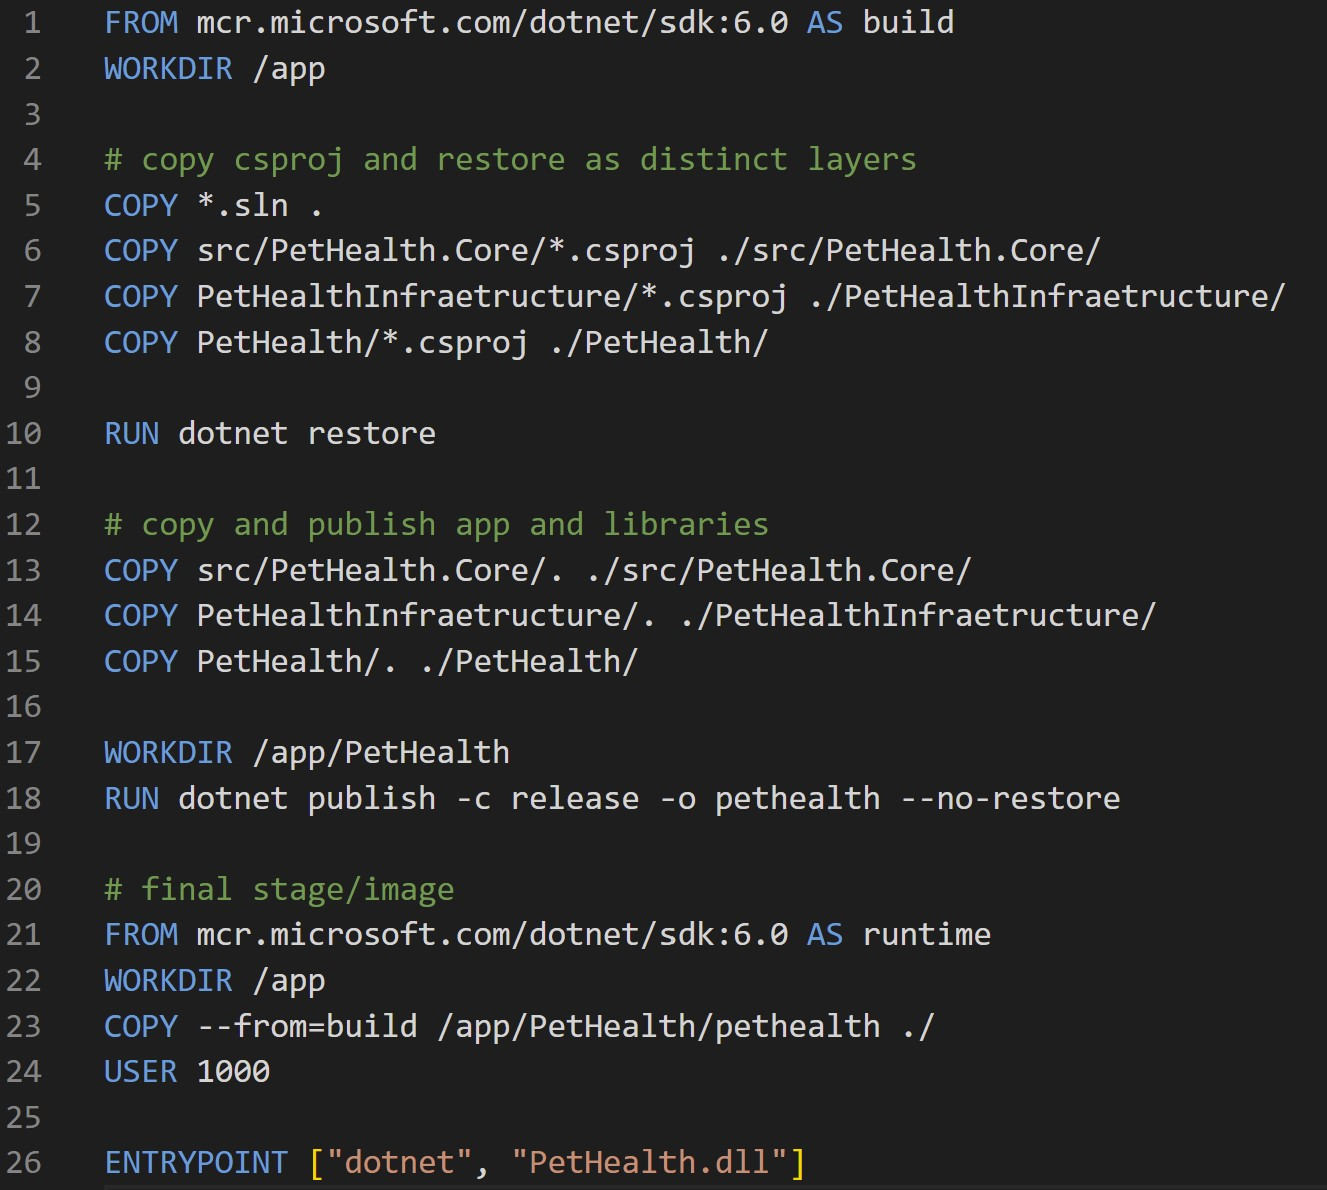
\includegraphics[width = 12cm, height=10cm]{Graphics/dokerfile.jpg}
	\caption{Dokerfile para .NET web api. }
	\label{fig:dockerfile}
\end{figure}

Como podemos ver hemos contenerizado nuestra aplicación en unos cuantos pasos y ya es un contenedor listo para ser ejecutado en cualquier máquina con una instalación de Docker.

\subsection{Mogenius:}

Mogenius es una herramienta web que automatiza todo el proceso de despliegue y de host de una aplicación. Tiene además la funcionalidad de crear automáticamente un pipeline de CI/CD(Continue Integration/ Continue Deployment), de esta forma nuestra aplicación puede ser fácilmente actualizada sin necesidad de llevar a cabo repetidamente el engorroso desplegar la aplicación. La única configuración necesaria es proveer un archivo dockerfile el cual contenga las instrucciones para contenerizar nuestra aplicación. Este servicio está conectado a una rama específica del repositorio del proyecto en Gitub, lo que significa que cada vez que sea actualizada la rama principal, la aplicación será desplegada automáticamente sin necesidad de interferir en el proceso. Otra de las ventajas de que el servicio esté conectado a Github, es que podemos controlar las versiones de la aplicación a través de comandos de Git.


\section{Detalles de implementación:}

\brackcite{marcotte2020atypical}En la ingeniería de software existen muchos conceptos de suma importancia para el desarrollo de soluciones robustas y flexibles. \textbf{SOLID} es el acrónimo atribuido a una serie de principios que extienden los conceptos básicos de programación orientada a objetos: abstracción, encapsulación, herencia y polimorfismo. Es importante destacar que no hablamos de reglas y una de las peores formas de aplicarlos es no adaptarlos a nuestro proyecto, o usarlos sin calcular si el beneficio del resultado de hacerlo. La correcta implementación del software marca la diferencia de un sistema que puede fácilmente actualizarse y mantenerse a la altura de los estándares del mercado, o uno que con el tiempo es simplemente muy costoso de mantener. Muchas son las formas de cumplir con las buenas prácticas del desarrollo de software. En este capítulo abordaremos algunas de las usadas por nosotros en el proceso de diseño y desarrollo de nuestra propuesta de producto.

\subsection{Datos:}

\brackcite{medina2017web}La capa de datos encargada de la persistencia está presente en cada proyecto que necesite persistir información de la aplicación. En la mayoría de los programas los datos son guardados en una base de datos. Al hablar de la capa de datos, dos de lo patrones de diseño más comunes son \textbf{Unit of Work} y  \textbf{Repository}.
\newline

El patrón Repository tiene como objetivo permitir lanzar consultas a la base de datos en forma de orientada a objetos. Entity Framework Core representa este concepto a través de \lstinline{DbSet<T>}  y permite filtrar estas consultas usando \textbf{LINQ} y la interfaz \lstinline{IQueryable<T>}. 

\begin{figure}[H]
	\centering
	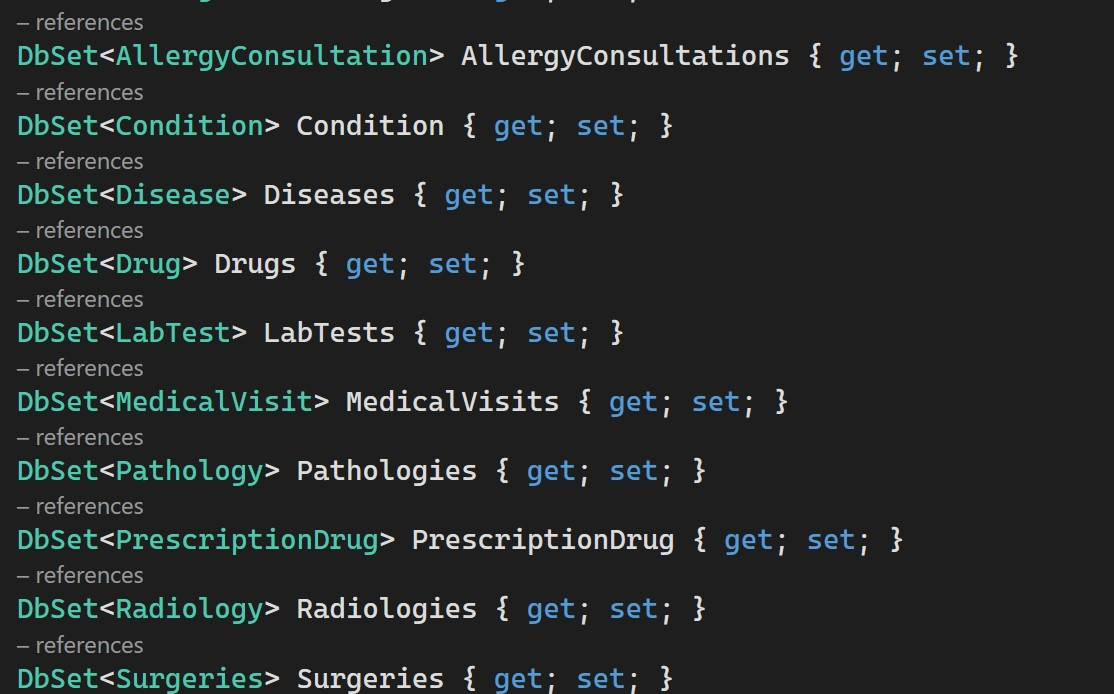
\includegraphics[width = 12cm, height=10cm]{Graphics/ef_core_repository_pattern.jpg}
	\caption{DbSet<T> para patrón Repository con EF Core.}
	\label{fig:EfCoreRepository}
\end{figure}

Es usual confundir el patrón de diseño \textbf{Repository} con el patrón \textbf{Table Data Gateaway}. Este último se usa para crear una abstracción del acceso a las tablas de la base de datos de una forma natural, permitiendo el uso de objetos más personalizados para interactuar con los datos. En la figura \ref{fig:tableDataGateaway} se puede ver nuestra implementación de este patrón. \brackcite{medina2017web}El \textbf{Table Data Gateaway} provee una encapsulación que sirve como puerta de enlace para acceder a los datos. Ofrece flexibilidad e independencia a la persistencia de la información ya que el patrón permite una total abstracción de las consultas SQL.

\begin{figure}[H]
	\centering
	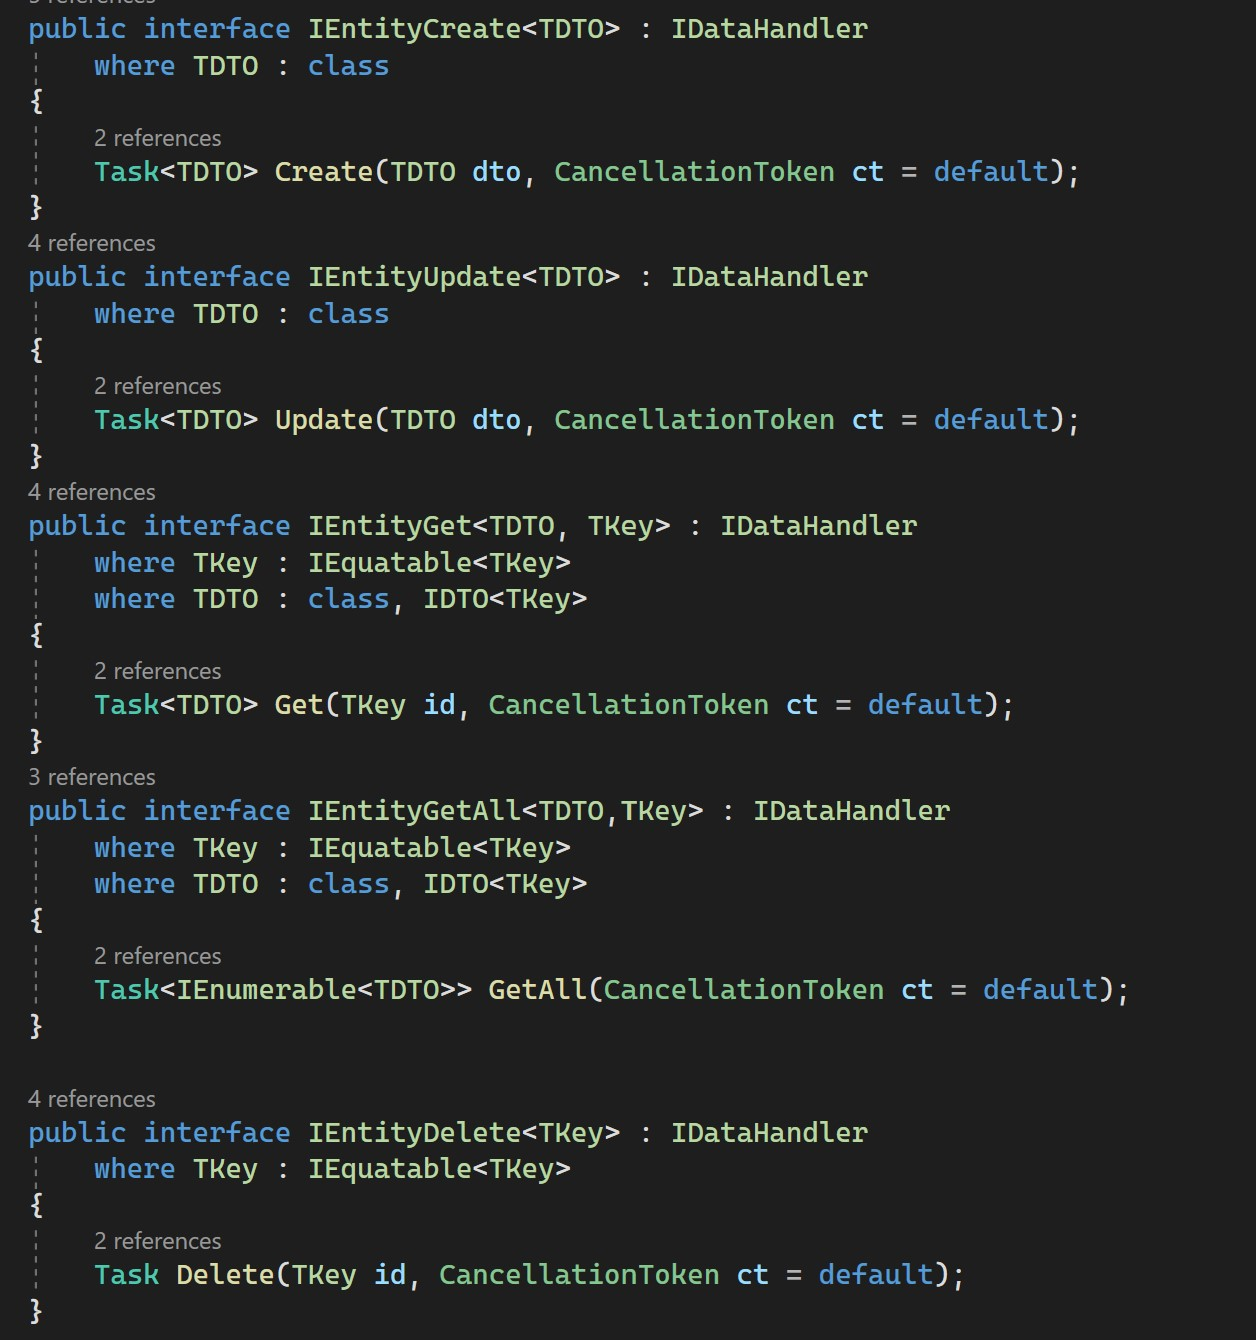
\includegraphics[width = 12cm, height=10cm]{Graphics/table_data_gateaway_pattern.jpg}
	\caption{Patrón de diseño Table Data Gateaway.}
	\label{fig:tableDataGateaway}
\end{figure}

\brackcite{marcotte2020atypical}Otro de los patrones importantes en el uso de datos, en especial desde una base de datos es \textbf{Unit of Work}. Este patrón permite seguir los cambios hechos en las entidades a las que accedemos en, agrupando además los cambios que deben ser enviados a la base de datos. En otras palabras, nos permite guardar y seguir en forma de objeto todas las transacciones que deben llevarse a cabo en la base de datos. La importancia de este patrón viene dada porque el acceso a la base de datos es siempre costoso y minimizar la cantidad de llamados que le hacemos es importante para el rendimiento de cualquier aplicación. La forma en la que este patrón funcione en Entity Framework Core es la siguiente:

\begin{enumerate}
	\item EF consulta la base de datos.
    \item Guarda las entidades devueltas en caché.
    \item Comienza a seguir los cambios hechos a estas entidades.
    \item Nos devuelve las entidades solicitadas en nuestra consulta.
    
\end{enumerate}


De esta forma EF crea una contexto para las entidades que sigue, guardando en este todas las transacciones que debe efectuar para aplicar los cambios detectados. Después de hacer cambios y crear transacciones sobre las entidades, haciendo un llamado al método \lstinline{SaveChanges()} de \lstinline{DbSet<T>} le decimos a EF Core que comience a ejecutar todas las transacciones detectadas. EF ejecuta esta acción de forma muy eficiente, ya que como mencionamos anteriormente realizará un solo llamado a la base de datos para aumentar la eficiencia de la comunicación con esta. Otras de las ventajas de este patrón es el manejo de errores, si alguna transacción falla entonces ninguna es aplicada, esto evita operaciones incompletas sobre la base de datos y la creación de datos inconsistentes. El siguiente método de nuestra aplicación permite ver un ejemplo donde se crean varias transacciones y se aplican al final guardando los cambios en el contexto.

\begin{lstlisting}
    public async Task SynchronizeSet(SynchroDataDTO synchroData, CancellationToken cancellationToken)
        {
            foreach (var entity in synchroData.Allergies)
            {
                Allergies temp = this._mapper.Map<Allergies>(entity);
                _context.Allergies.Add(temp);
            }

            foreach (var allergyCons in synchroData.AllergyConsultation)
            {
                AllergyConsultation temp = this._mapper.Map<AllergyConsultation>(allergyCons);
                _context.AllergyConsultations.Add(temp);
            }

            foreach (var condition in synchroData.Condition)
            {
                Condition temp = this._mapper.Map<Condition>(condition);
                _context.Condition.Add(temp);
            }

            foreach (var disease in synchroData.Disease)
            {
                Disease temp = this._mapper.Map<Disease>(disease);
                _context.Diseases.Add(temp);
            }

            foreach (var drug in synchroData.Drug)
            {
                Drug temp = this._mapper.Map<Drug>(drug);
                _context.Drugs.Add(temp);
            }

            foreach (var labTest in synchroData.LabTest)
            {
                LabTest temp = this._mapper.Map<LabTest>(labTest);
                _context.LabTests.Add(temp);
            }

            foreach (var medicalVisit in synchroData.MedicalVisit)
            {
                MedicalVisit temp = this._mapper.Map<MedicalVisit>(medicalVisit);
                _context.MedicalVisits.Add(temp);
            }

            foreach (var note in synchroData.Note)
            {
                Note temp = this._mapper.Map<Note>(note);
                _context.Notes.Add(temp);
            }

            foreach (var pathology in synchroData.Pathology)
            {
                Pathology temp = this._mapper.Map<Pathology>(pathology);
                _context.Pathologies.Add(temp);
            }

            foreach (var radiology in synchroData.Radiology) 
            {
                Radiology temp = this._mapper.Map<Radiology>(radiology);
                _context.Radiologies.Add(temp);
            }

            foreach (var surgeries in synchroData.Surgeries) 
            {
                Surgeries temp = this._mapper.Map<Surgeries>(surgeries);
                _context.Surgeries.Add(temp);
            }

            foreach (var prescriptionDrug in synchroData.PrescriptionDrug)
            {
                PrescriptionDrug temp = this._mapper.Map<PrescriptionDrug>(prescriptionDrug);
                _context.PrescriptionDrug.Add(temp);
            }

            foreach (var vaccine in synchroData.Vaccines)
            {
                Vaccines temp = this._mapper.Map<Vaccines>(vaccine);
                _context.Vaccines.Add(temp);
            }

            foreach (var vaccineConsultation in synchroData.VaccineConsultation)
            {
                VaccineConsultation temp = this._mapper.Map<VaccineConsultation>(vaccineConsultation);
                _context.VaccineConsultations.Add(temp);
            }

          await _context.SaveChangesAsync(cancellationToken);
        }
\end{lstlisting}

\subsection{Inyección de Dependencia:}
\brackcite{marcotte2020atypical}La inyección de dependencias es una de las formas de implementar el principio de inversión de control de \textbf{SOLID}, es la \textbf{D} en este acrónimo. Podemos entender el principio de inversión de control como una versión más amplia de la inyección de dependencias. La idea principal es dejar la creación de dependencias al punto de entrada del programa. De esta forma el manejo de dependencias es hecho por un contenedor de inversión de control y los desarrolladores pueden abstraerse de esto cuando realizan sus implementaciones. 
\newline
En \textbf{.NET} tenemos la clase \lstinline{WebApplicationBuilder}, esta se encarga, entre otras cosas, de registrar las dependencias que usaremos en nuestra aplicación para que estas puedan ser resueltas a medida que son demandadas. A continuación se ve un ejemplo de como registrar una dependencia y seguido el constructor de una clase que usa esta dependencia abstrayéndose de la forma de obtenerla.


\begin{figure}[H]
	\centering
	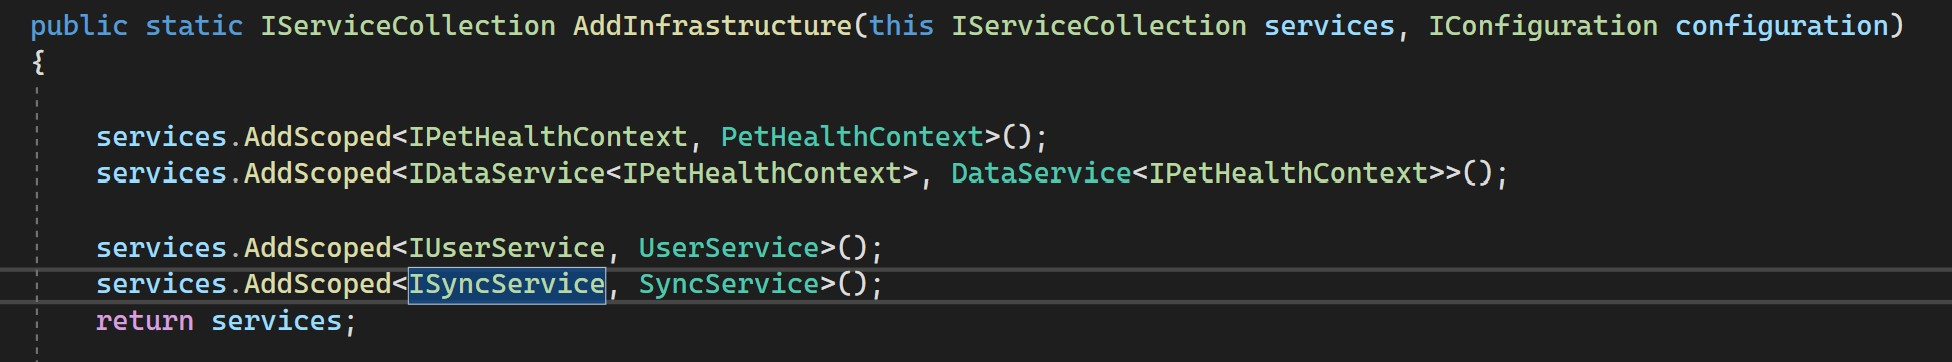
\includegraphics[width = 12cm]{Graphics/di_register_example.jpg}
	\caption{Registro de Inyección de Dependencia en .NET.}
	\label{fig:di_register}
\end{figure}

\begin{figure}[H]
	\centering
	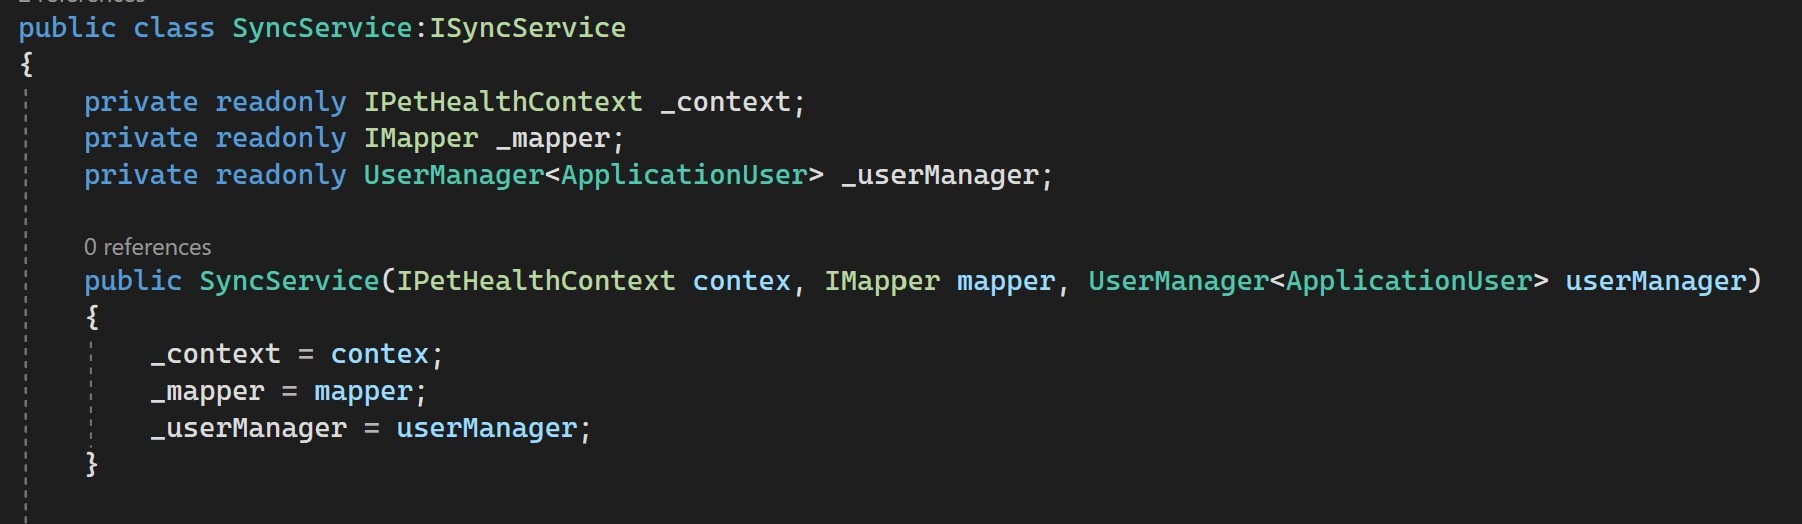
\includegraphics[width = 12cm]{Graphics/dep_inj_example.jpg}
	\caption{Uso de Inyección de Dependencia en un constructor en .NET.}
	\label{fig:di_use_example}
\end{figure}

Existen gran variedad de patrones de diseño y principios de arquitectura que son usados en una aplicación, todos de suma importancia cuando se quiere entregar software de buena calidad. En este pequeño apartado hemos abordado solo algunas que consideramos tienen un gran impacto tanto en la calidad del proceso de desarrollo como en la del producto final. Podemos asegurar que es perceptible la fluidez del desarrollo de software cuando se aplican estos principios y patrones. También creemos necesario hacer hincapié en la importancia de adaptarlos a nuestro producto. Estos patrones y principios por sí solos, sin análisis de su uso en nuestro producto pueden resultar en un problema considerablemente grande en su diseño e implementación.

\section{Conlusión:}
En este capítulo hacemos un análisis de las tecnologías y herramientas usadas para el desarrollo de nuestra aplicación. Principalmente podemos destacar el papel protagonista de las librerías de acceso a datos. Estas tecnologías han demostrado ser fundamentales tanto para el desarrollo correcto de aplicaciones como para la entrega de soluciones robustas y eficientes. También se analizó el impacto que tiene una estrategia de despliegue cómoda y segura del software. Además se pudo apreciar las ventajas que nos da la contenerización de software y lo fácil que puede ser integrarlo en nuestras estrategias de desarrollo de software.  Cerramos el capítulo con una observación sobre elementos de ingeniería que eran necesarios destacar por su impacto positivo en el logro de un software robusto.